\documentclass[11pt,a4paper]{ctexart}
% 调整页面大小,默认页面与常用规格不符
\usepackage[margin=1in,top=1.5in]{geometry}
\pagestyle{headings}
\usepackage[utf8]{inputenc}

\usepackage{float}

% 插入数学及电学符号
\usepackage{amsmath}
\usepackage{amsfonts}
\usepackage{amssymb}

% 插入附件
\usepackage{navigator}

% 引用链接可点击
\usepackage{cite}
\usepackage[colorlinks,linkcolor=black,anchorcolor=blue,citecolor=green]{hyperref}

% 插入图片
\usepackage{graphicx}

% 绘制各种图形,包括电路图,函数图
\usepackage{tikz}
\usepackage{pgfplots}

\makeatletter
\newcommand\dlmu[2][4cm]{\hskip1pt\underline{\hb@xt@ #1{\hss#2\hss}}\hskip3pt}
\makeatother


% 标题居左 显示成如下情况 一、标题
\ctexset{
section={
name={第,章},
number=\arabic{section},
format=\Large\bfseries\raggedright\heiti
},
}

% 设置页眉
\usepackage{fancyhdr}
\pagestyle{fancy}
\fancyhf{} % 清空当前的页眉页脚
\fancyhead[C]{\heiti 数据结构实验报告}

% 用于插入C代码
\usepackage{listings}


% 调整代码的背景和风格
\usepackage{xcolor}
\lstset{
%行号
numbers=left,
%背景框
framexleftmargin=10mm,
frame=none,
%背景色
%backgroundcolor=\color[rgb]{1,1,0.76},
backgroundcolor=\color[RGB]{245,245,244},
%样式
keywordstyle=\bf\color{blue},
identifierstyle=\bf,
numberstyle=\color[RGB]{0,192,192},
commentstyle=\it\color[RGB]{0,96,96},
stringstyle=\rmfamily\slshape\color[RGB]{128,0,0},
%显示空格
showstringspaces=false
}


\bibliographystyle{plain}

\numberwithin{figure}{section}


\begin{document}
    \heiti
    \begin{titlepage}
        \centering
        \rule[1.10cm]{\linewidth}{0cm}

        
\includegraphics[width=0.4\linewidth]{figures/Banner}

        \vspace{0.5cm}
        \textbf{\zihao{0} 实验报告}

        \vspace{1cm}
        \textbf{{\Huge 线性表的链式存储结构与应用}}

        \begin{LARGE}
            \vspace{2cm}
            班\rule{38pt}{0pt}级 \dlmu[6cm]{1603002}\\ \vspace{4pt}
            学\rule{38pt}{0pt}号 \dlmu[6cm]{1160300202}\\ \vspace{4pt}
            姓\rule{38pt}{0pt}名 \dlmu[6cm]{冯云龙}\\ \vspace{4pt}
            指导教师 \dlmu[6cm]{张岩}\\ \vspace{4pt}
            实验日期 \dlmu[6cm]{2017/10/31}\\ \vspace{4pt}
            设计成绩 \dlmu[6cm]{}\\ \vspace{4pt}
            报告成绩 \dlmu[6cm]{}\\ \vspace{4pt}
        \end{LARGE}

        \vfill
        {\huge \textbf{计算机科学与技术学院}}
        % 底部插入当日日期
    \end{titlepage}

    \tableofcontents
    \newpage
    \section{实验目的}
树型结构的建立与遍历。

\section{实验要求及实验环境}
\subsection{实验要求}
\begin{enumerate}
    \item 设计 AVL 的左右链存储结构;
    \item 实现 AVL 左右链存储结构上的插入(建立)、删除、查找和排序算法。
    \item 测试数据以文件形式保存,能反映插入和删除操作的四种旋转,并输出相应的结果。
\end{enumerate}

\subsection{实验环境}
\subsubsection{硬件环境}
\begin{itemize}
    \item CPU: Intel Core i7-6700HQ @ 8x 3.5GHz
    \item RAM: 3516MiB / 7899MiB
\end{itemize}

\subsubsection{软件环境}
\begin{itemize}
    \item Manjaro Linux
\end{itemize}

\subsubsection{开发工具}
\begin{itemize}
    \item GCC
    \item Clion
\end{itemize} %实验目的 实验要求及实验环境
    \section{Y86-64顺序处理器设计}
\begin{center}
    (该章满分50分)
\end{center}

\subsection{Y86-64顺序处理器结构设计}

\begin{figure}[H]
\centering
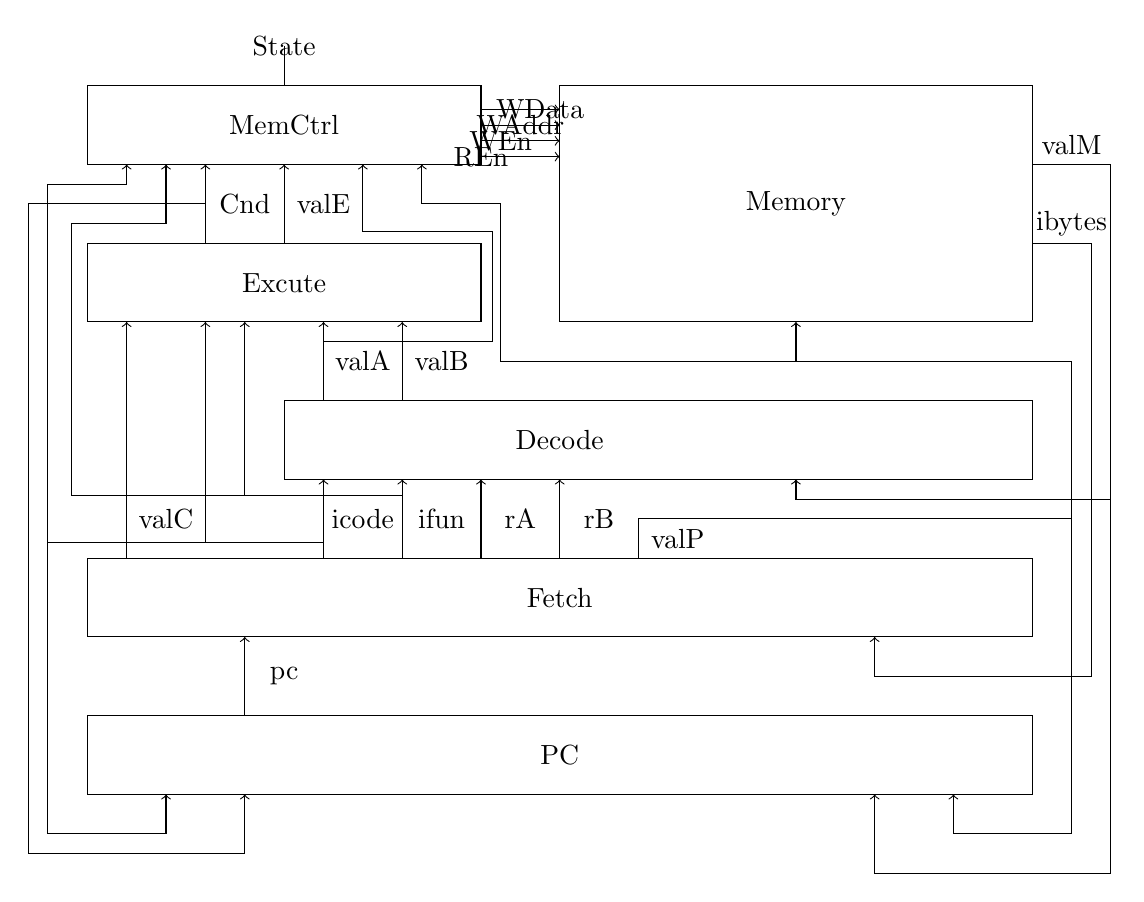
\begin{tikzpicture}
    \draw (0,0) rectangle +(12,1);
    \draw (6,0.5) node{PC};
    
    \draw (0,2) rectangle +(12,1);
    \draw (6,2.5) node{Fetch};
    
    \draw (2.5,4) rectangle +(9.5,1);
    \draw (6,4.5) node{Decode};
    
    \draw (0,6) rectangle +(5,1);
    \draw (2.5,6.5) node{Excute};
    
    \draw (0,8) rectangle +(5,1);
    \draw (2.5,8.5) node{MemCtrl};
    
    \draw (6,6) rectangle +(6,3);
    \draw (9,7.5) node{Memory};

%pc
    \draw [->](2,1) -- (2,2);
    \draw (2.5,1.5) node{pc};
    
%fetch
    \draw [->](3,3) -- (3,4);
    \draw [->](3,3.2) -- (1.5,3.2) -- (1.5,6);
    \draw [->](3,3.2) -- (-0.5,3.2) -- (-0.5,-0.5) -- (1,-0.5) -- (1,0);
    \draw [->](-0.5,3.2) -- (-0.5,7.75) -- (0.5,7.75) -- (0.5,8);
    \draw (3.5,3.5) node{icode};
    
    \draw [->](4,3) -- (4,4);
    \draw [->](4,3.8) -- (2,3.8) -- (2,6);
    \draw [->](4,3.8) -- (-0.2,3.8) -- (-0.2,7.25) -- (1,7.25) -- (1,8);
    \draw (4.5,3.5) node{ifun};
    
    \draw [->](5,3) -- (5,4);
    \draw (5.5,3.5) node{rA};
    
    \draw [->](6,3) -- (6,4);
    \draw (6.5,3.5) node{rB};
    
    \draw [->](0.5,3) -- (0.5,6);
    \draw (1,3.5) node{valC};
    
    \draw [->](7,3) -- (7,3.5) -- (12.5,3.5) -- (12.5,3.5) -- (12.5,-0.5) -- (11,-0.5) -- (11,0);
    \draw [->](12.5,3.5) -- (12.5,5.5) -- (5.25,5.5) -- (5.25,7.5) -- (4.25,7.5)--(4.25,8);
    \draw [->](9,5.5)--(9,6);
    \draw (7.5,3.25) node{valP};
    
%decode
    \draw [->](3,5) -- (3,6);
    \draw [->](3,5.75) -- (5.15,5.75) -- (5.15,7.15) -- (3.5,7.15) -- (3.5,8);
    \draw (3.5,5.5) node{valA};
    
    \draw [->](4,5) -- (4,6);
    \draw (4.5,5.5) node{valB};
    
%execute
    \draw [->](1.5,7) -- (1.5,8);
    \draw [->](1.5,7.5) -- (-0.75,7.5) -- (-0.75,-0.75) -- (2,-0.75) --(2,0);
    \draw (2,7.5) node{Cnd};
    
    \draw [->](2.5,7) -- (2.5,8);
    \draw (3,7.5) node{valE};
    
%memctrl
    \draw [->] (5,8.1) -- (5.0,8.1)node{REn} -- (6,8.1);
    \draw [->] (5,8.3) -- (5.25,8.3)node{WEn} -- (6,8.3);
    \draw [->] (5,8.5) -- (5.5,8.5)node{WAddr} -- (6,8.5);
    \draw [->] (5,8.7) -- (5.75,8.7)node{WData} -- (6,8.7);
    \draw (2.5,9) -- (2.5,9.5) node{State};
    
%memory
    \draw [->] (12,7) -- (12.75,7) -- (12.75,1.5) -- (10,1.5)--(10,2);
    \draw (12.5,7.25) node{ibytes};
    \draw [->] (12,8) -- (13,8) -- (13,-1) --(10,-1) -- (10,0);
    \draw [->] (13,3.75)--(9,3.75)--(9,4);
    \draw (12.5,8.25)node{valM};

\end{tikzpicture}
\caption{Y86-64处理器结构}
\end{figure}

\subsection{Y86-64顺序处理器模块设计(包含Verilog模块接口设计)}

\subsubsection{PC}
\begin{minted}{verilog}
module PC(
    input clock,
    input  [3:0] icode,
    input  Cnd,
    input  [63:0] ValM,
    input  [63:0] ValC,
    input  [63:0] ValP,
    output reg[63:0] pc,
    input reset
);
\end{minted}

根据icode和cnd对PC进行更新。

\subsubsection{取指}
\begin{minted}{verilog}
module Fetch(
    input [63:0] pc,
    input [79:0] ibytes,
    input imem_error,
    output instr_valid,
    output [3:0] icode,
    output [3:0] ifun,
    output [3:0] rA,
    output [3:0] rB,
    output [63:0] valC,
    output [63:0] valP
);
\end{minted}

对传入的ibytes进行解析,拆分成icode,ifun,rA,rb,valC,并根据拆分值计算valP。


\subsubsection{译码}
\begin{minted}{verilog}
module Decode(
    input clock,
    input [3:0] icode,
    input [3:0] rA,
    input [3:0] rB,
    input cnd,
    input [63:0] valM,
    input [63:0] valE,
    output [63:0] valA,
    output [63:0] valB
);
\end{minted}

传入rA、rB、icode、Cnd,根据icode的值和Cnd的值读出寄存器的值并对寄存器文件进行写入。

\subsubsection{执行}
\begin{minted}{verilog}
module Excute(
    input clock,
    input  [3:0] icode,
    input  [3:0] ifun,
    input  [63:0]valC,
    input  [63:0]valA,
    input  [63:0]valB,
    input  reset,
    output Cnd,
    output [63:0]valE
);
\end{minted}

根据指令icode进行数据运算,并更新Cnd。

\subsubsection{访存}
\begin{minted}{verilog}
module MemCtrl(
    input [3:0]icode,
    input [63:0]valE,
    input [63:0]valA,
    input [63:0]valP,
    input instr_valid,
    input im_error,
    input dm_error,
    output readEn,
    output writeEn,
    output [1:0]status,
    output [63:0]mem_addr,
    output [63:0]mem_data
);
\end{minted}

根据icode的值决定内存读信号和内存写信号,以及内存地址的取值和写入内存的数据。该模块与Bmemory模块连接,控制内存的读写,同时输出处理器运行状态。

\begin{minted}{verilog}
module BMemory(
    input clock,
    input read,
    input write,
    input [63:0] maddr,
    input [63:0] wdata,
    output [63:0] rdata, //valM
    input [63:0] iaddr,
    output [79:0] idata,
    output i_ok,
    output m_ok
);
\end{minted}

根据内存控制信号执行相应操作。如果内存读信号为1,则通过内存地址按字节依次取出该数据存入寄存器,如果内存写信号为1,则把要写入内存的数据写入内存。

\subsubsection{处理器}
\begin{minted}{verilog}
module Processor(
    input [2:0] mode,
    input [63:0] udaddr,
    input [63:0] idata,
    input clock
);
\end{minted}

对各个模块进行综合,形成完整的处理器,这里可以通过改变状态对内存进行读写操作。
 %设计思想
    \section{设计验证}
\begin{center}
    (该章满分20分)
\end{center}

\subsection{仿真验证}

选取2.3节中的任意两条机器指令,给出机器码格式,建立testbench文件,进行波形仿真。给出测试结果(波形图需要截屏)。

这里所给出的Processor已经被修改过了,主要是为了可以直观的看到执行机器码之后对寄存器的修改。

\begin{minted}{gas}
30f20a00000000000000 |   irmovq $10,%rdx
30f00300000000000000 |   irmovq  $3,%rax
6020                 |   addq %rdx,%rax
\end{minted}

\begin{minted}{verilog}
module testbench( );
    parameter RUN_MODE = 2'h0;
    parameter RESET_MODE = 2'h1;
    parameter DOWNLOAD_MODE = 2'h2;
    parameter UPLOAD_MODE = 2'h3;
    
    reg clock = 0;
    reg [2:0] mode = RESET_MODE;
    reg [63:0]uaddr = 0;
    reg [63:0]idata = 1;
    wire [63:0]rax;
    wire [63:0]rdx;
    
    always begin
        clock = 1;
        # 5;
        clock = 0;
        # 5;
    end
    
    //30f20a00000000000000 |   irmovq $10,%rdx
    //30f00300000000000000 |   irmovq  $3,%rax
    //6020                 |   addq %rdx,%rax
    
    initial begin
    #20 mode <= DOWNLOAD_MODE;
    uaddr <= 0;
    idata <= 64'h00000000000af230;
    #20;
    uaddr <= 8;
    idata <= 64'h00000003f0300000;
    #20;
    uaddr <= 16;
    idata <= 64'h000206000000000;
    #20;
    uaddr <= 24;
    idata <= 64'h0000000000000000;
    #20 mode <= RESET_MODE;
    #20 mode <= RUN_MODE;
    end
    
    Processor p(mode,uaddr,idata,rax,rdx,clock);

endmodule
\end{minted}

\begin{figure}
    \centering
    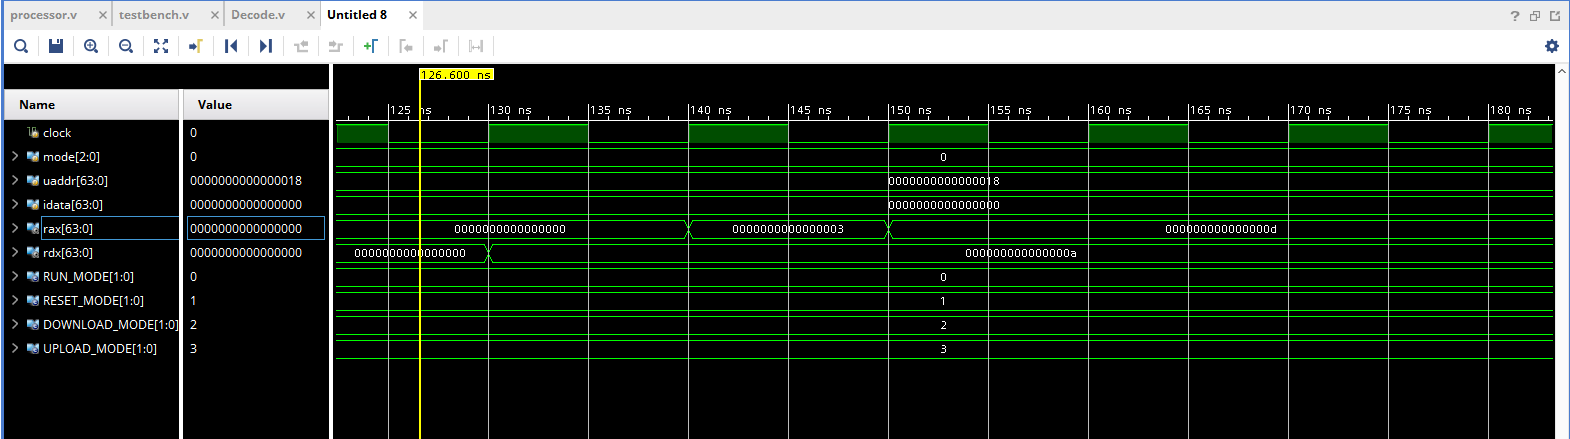
\includegraphics[width=0.7\linewidth]{figures/Sim}
    \caption{仿真波形}
    \label{fig:sim}
\end{figure}


\subsection{综合(synthesis)验证}
\begin{center}
    (选做,加分项,最多加分值为作业项总成绩的5分,作业项分值加满为止)
\end{center}

以2.3节中的程序为例,写出对应机器码格式,在某FPGA实验台上验证。

\section{总结}
\subsection{请总结本次实验的收获}
\begin{enumerate}
    \item 重新复习了vivado和verilog相关知识
    \item 对CPU顺序处理器的内部结构和运转过程有了更加深入的了解
    \item 在对SEQ不断修改调整的过程中加深了对CPU功能及与内存关系的理解
\end{enumerate}

\subsection{请给出对本次实验内容的建议}
希望可以第一时间给出参考资料。 %测试结果
    \section{BITS函数实验与分析}
\begin{center}
    每题8分,总分不超过80分
    截图:  \$ ./btest –f 函数名
\end{center}

\subsection{函数lsbZero的实现及说明}

\paragraph{程序如下:}
\begin{minted}{c}
int lsbZero(int x) {
    return x & ((1 << 31) >> 30);
}
\end{minted}

\begin{figure}[H]
\begin{minipage}[c]{0.5\linewidth}
\paragraph{设计思想:}主要考虑获得0xfffffffe,即处lsb为0外,其他位全部为1的值与x相与。
\end{minipage}
\begin{minipage}[c]{0.4\linewidth}
\centering
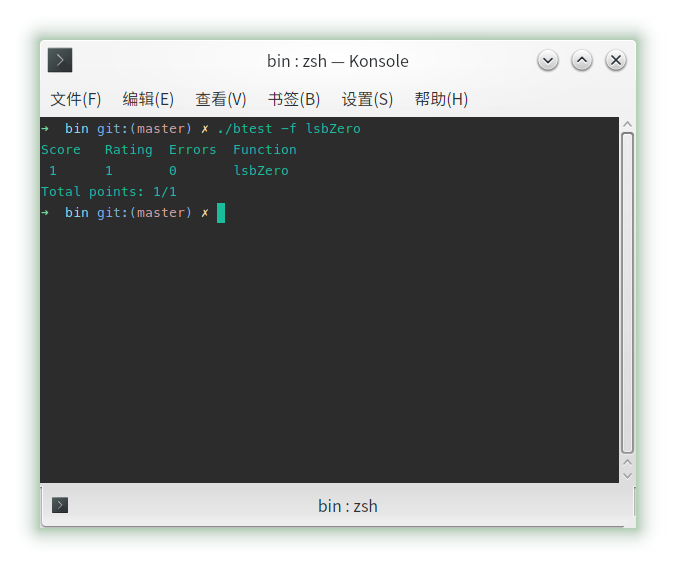
\includegraphics[width=0.9\linewidth]{figures/lsbZero}
\caption{btest截图-lsbZero}
\label{fig:lsbzero}
\end{minipage}
\end{figure}

\subsection{函数byteNot的实现及说明}

\textbf{程序如下:}
\begin{minted}{c}
int byteNot(int x, int n) {
    return x ^ (0xFF << (n << 3));
}
\end{minted}

\begin{figure}[H]
\begin{minipage}[c]{0.5\linewidth}
\textbf{设计思想:}发现数值与1异或可以取反,将需要取反的字节的与0xff对齐进行异或即可。    
\end{minipage}
\begin{minipage}[c]{0.4\linewidth}
\centering
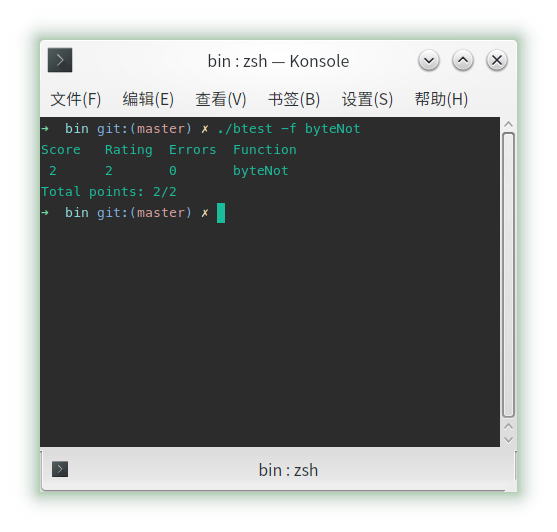
\includegraphics[width=0.9\linewidth]{figures/byteNot}
\caption{btest截图-byteNot}
\label{fig:byteNote}
\end{minipage}
\end{figure}

\subsection{函数byteXor的实现及说明}

\textbf{程序如下:}
\begin{minted}{c}
int byteXor(int x, int y, int n) {
    return !(!(0xFF & ((x ^ y) >> (n << 3))));
}
\end{minted}

\begin{figure}[H]
\begin{minipage}[c]{0.5\linewidth}
        
\textbf{设计思想:}简单考虑,对所有位进行异或比较,然后取得所需要的字节部分的结果即可,使用两次逻辑取非,获得逻辑值。
        
\end{minipage}
\begin{minipage}[c]{0.4\linewidth}
\centering
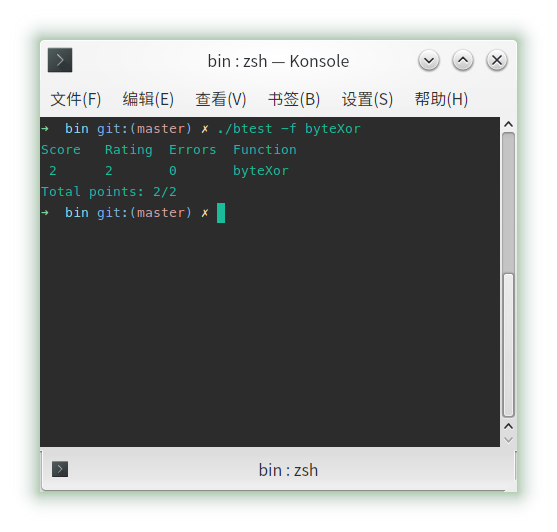
\includegraphics[width=0.9\linewidth]{figures/byteXor}
\caption{btest截图-byteXor}
\label{fig:byteXor}
\end{minipage}
\end{figure}

\subsection{函数logicalAnd的实现及说明}
\textbf{程序如下:}
\begin{minted}{c}
int logicalAnd(int x, int y) {
    return !(!x | !y);
}
\end{minted}

\begin{figure}[H]
\begin{minipage}[c]{0.5\linewidth}
\textbf{设计思想:}使用逻辑非取得输入值的逻辑值,再进行位运算即可获得逻辑结果。
        
\end{minipage}
\begin{minipage}[c]{0.4\linewidth}
\centering
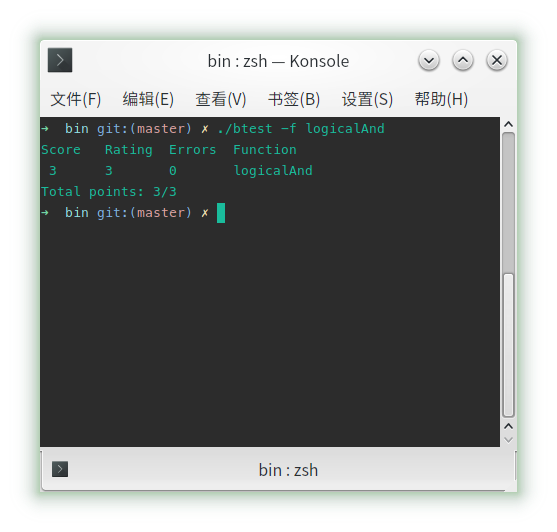
\includegraphics[width=0.9\linewidth]{figures/logicalAnd}
\caption{btest截图-logicalAnd}
\label{fig:logicalAnd}
\end{minipage}
\end{figure}

\subsection{函数logicalOr的实现及说明}
\textbf{程序如下:}

\begin{minted}{c}
int logicalOr(int x, int y) {
    return !(!x & !y);
}
\end{minted}

\begin{figure}[H]
\begin{minipage}[c]{0.5\linewidth}
\textbf{设计思想:}使用逻辑非取得输入值的逻辑值,再进行位运算即可获得逻辑结果。
        
\end{minipage}
\begin{minipage}[c]{0.4\linewidth}
\centering
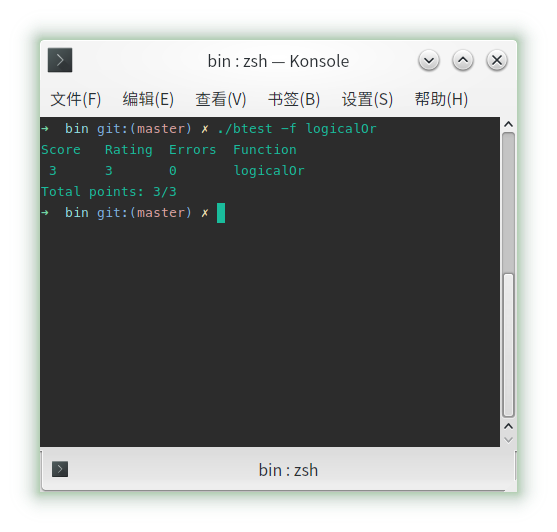
\includegraphics[width=0.9\linewidth]{figures/logicalOr}
\caption{btest截图-logicalOr}
\label{fig:logicalOr}
\end{minipage}
\end{figure}

\subsection{函数rotateLeft的实现及说明}
\textbf{程序如下:}
    
\begin{minted}{c}
int rotateLeft(int x, int n) {
    int N_31 = ~n + 33;
    return (x << n) | (~(~0x00 << n) & (x >> N_31));
}
\end{minted}
    
\begin{figure}[H]
\begin{minipage}[c]{0.5\linewidth}
\textbf{设计思想:}重点是发现 \mintinline{c}|-a=~a+1|,之后将数据位进行移动,使用掩码做多余数据消除,而后合并。
\end{minipage}
\begin{minipage}[c]{0.4\linewidth}
\centering
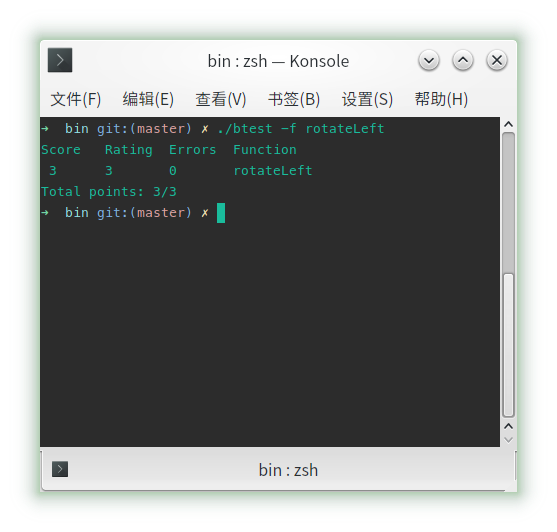
\includegraphics[width=0.9\linewidth]{figures/rotateLeft}
\caption{btest截图-rotateLeft}
\label{fig:rotateLeft}
\end{minipage}
\end{figure}

\subsection{函数parityCheck的实现及说明}

\textbf{程序如下:}

\begin{minted}{c}
int parityCheck(int x) {
    x = (x >> 16) ^ x;
    x = (x >> 8) ^ x;
    x = (x >> 4) ^ x;
    x = (x >> 2) ^ x;
    x = (x >> 1) ^ x;
    return x & 0x01;
}
\end{minted}

\begin{figure}[H]
    \begin{minipage}[c]{0.5\linewidth}
        \textbf{设计思想:}使用归并的思路进行各位的比较,若为偶数个1,最终会被全部抵消。
    \end{minipage}
    \begin{minipage}[c]{0.4\linewidth}
        \centering
        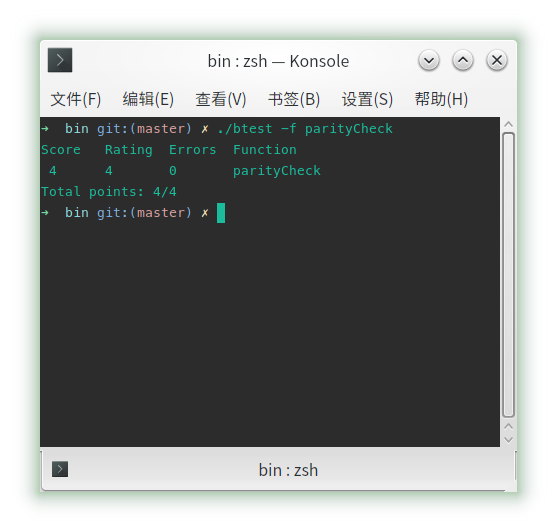
\includegraphics[width=0.9\linewidth]{figures/parityCheck}
        \caption{btest截图-parityCheck}
        \label{fig:parityCheck}
    \end{minipage}
\end{figure}

\subsection{函数mul2OK的实现及说明}
\textbf{程序如下:}

\begin{minted}{c}
int mul2OK(int x) {
    return (0x01 & ~((x >> 31) ^ (x >> 30)));
}
\end{minted}

\begin{figure}[H]
\begin{minipage}[c]{0.5\linewidth}
\textbf{设计思想:}主要是判断符号位是否发生了改变,若发生则是发生了溢出。
\end{minipage}
\begin{minipage}[c]{0.4\linewidth}
\centering
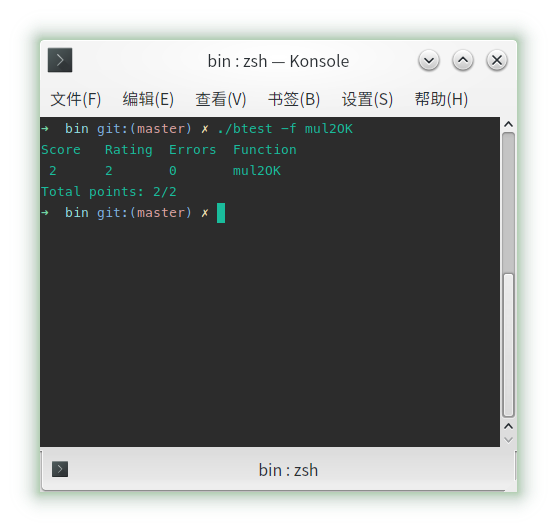
\includegraphics[width=0.9\linewidth]{figures/mul2OK}
\caption{btest截图-mul2OK}
\label{fig:mul2OK}
\end{minipage}
\end{figure}

\subsection{函数mult3div2的实现及说明}
\begin{minted}{c}
int mult3div2(int x) {
    int xmult3 = (x << 1) + x;
    return (xmult3 >> 1) + (((xmult3 >> 31) & 1) & (((xmult3 << 31) >> 31) & 1));
}
\end{minted}

\begin{figure}[H]
    \begin{minipage}[c]{0.5\linewidth}
        \textbf{设计思想:}左移一位再加$x$即$x*3$,右移一位即得$(x*3)/2$,当$x*3$的最高位和最低位都为0时需要+1。
    \end{minipage}
    \begin{minipage}[c]{0.4\linewidth}
        \centering
        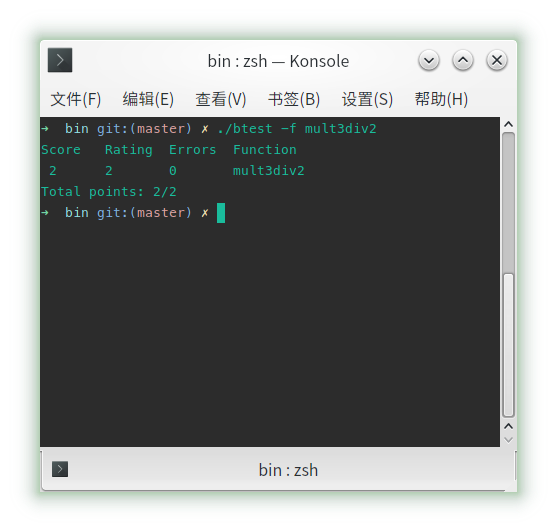
\includegraphics[width=0.9\linewidth]{figures/mult3div2}
        \caption{btest截图-mult3div2}
        \label{fig:mult3div2}
    \end{minipage}
\end{figure}

\subsection{函数subOK的实现及说明}

\begin{minted}{c}
int subOK(int x, int y) {
  int samesign = ((x ^ y) >> 31) & 0x01;
  return !(samesign & ((((x + ~y + 1) ^ x) >> 31) & 0x01));
}
\end{minted}

\begin{figure}[H]
    \begin{minipage}[c]{0.5\linewidth}
        \textbf{设计思想:}重点是注意到两个数符号相同时不会产生溢出,当符号不同时,减数的符号位参加运算则是发生了溢出。
    \end{minipage}
    \begin{minipage}[c]{0.4\linewidth}
        \centering
        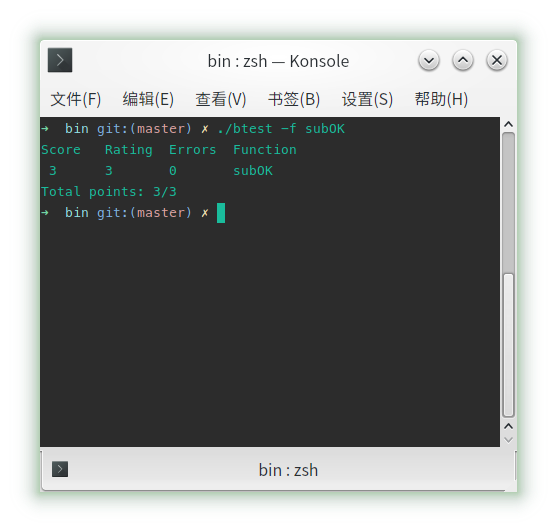
\includegraphics[width=0.9\linewidth]{figures/subOK}
        \caption{btest截图-subOK}
        \label{fig:subOK}
    \end{minipage}
\end{figure}

\subsection{函数absVal的实现及说明}
\textbf{程序如下:}

\begin{minted}{c}
int absVal(int x) {
  return ((x >> 31) & (~(x + ~0))) | (~(x >> 31) & x);
}
\end{minted}

\begin{figure}[H]
\begin{minipage}[c]{0.5\linewidth}
\textbf{设计思想:}若为正则不做处理,若为负则进行\mintinline{c}|-a=~a+1|的逆运算,通过符号位的判断决定取得的值。
\end{minipage}
\begin{minipage}[c]{0.4\linewidth}
\centering
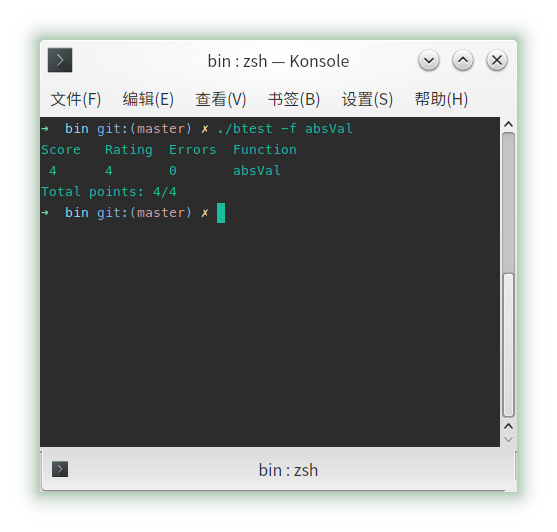
\includegraphics[width=0.9\linewidth]{figures/absVal}
\caption{btest截图-absVal}
\label{fig:absVal}
\end{minipage}
\end{figure}

\subsection{函数float\_abs的实现及说明}
\textbf{程序如下:}

\begin{minted}{c}
unsigned float_abs(unsigned uf) {
    unsigned sign = uf >> 31;
    unsigned exp = uf >> 23 & 0xFF;
    unsigned frac = uf & 0x7FFFFF;
    return uf & 0x7fffffff + (sign * ((exp == 0xFF && frac) << 31));
}
\end{minted}

\begin{figure}[H]
\begin{minipage}[c]{0.5\linewidth}
\textbf{设计思想:}符号位置零,若发现该数值为NaN则将符号位重新补上。
\end{minipage}
\begin{minipage}[c]{0.4\linewidth}
\centering
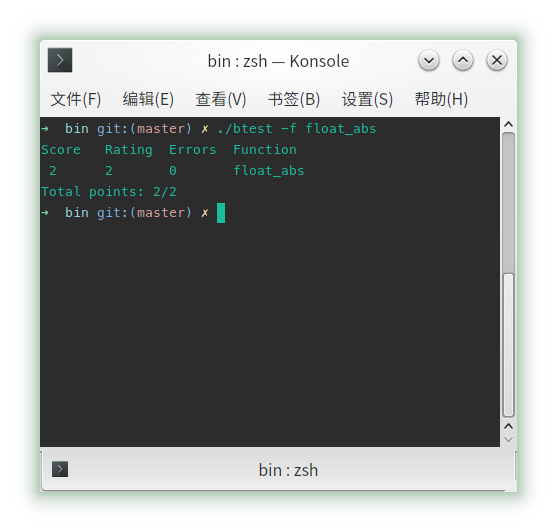
\includegraphics[width=0.9\linewidth]{figures/float_abs}
\caption{btest截图-float-abs}
\label{fig:float-abs}
\end{minipage}
\end{figure}

%\subsection{函数float\_f2i的实现及说明}
%\subsection{函数XXXX的实现及说明函数(CMU多出来的函数-不加分)}


 %经验体会与不足
    \appendix

\section{源代码}

\lstinputlisting[language = c++]{../AvlTree.h}
\lstinputlisting[language = c++]{../AvlMain.cpp}

    %附录:源代码

\end{document}